\section{Introduction}

\subsection{History}

This package was born out of a $\approx$~10 line function I wrote to estimate the memory usage of (non-allocated) in-core, dense \proglang{R} objects of numeric (double precision) data.  I need this in my life by a surprising amount, so it made sense to actually create this thing instead of constantly doing ad hoc multiplications of $nrows\times ncols \times 8$ then dividing by powers of $1024$ (or 1000).

But then I got the great idea to make this application \twiddle{enterprise ready} by adding a lot of unnecessary and convoluted OOP, and this stupid package was born.  This is sort of a love letter to other needlessly complex programs, like the \href{https://github.com/Mikkeren/FizzBuzzEnterpriseEdition}{Enterprise Fizzbuzz}\footnote{If you are unfamiliar with the \href{https://en.wikipedia.org/wiki/Bizz_buzz}{fizzbuzz}, see my posts ``\href{http://librestats.com/2012/01/10/honing-your-r-skills-for-job-interviews/}{Honing your R skills for Job Interviews}'' and ``\href{http://librestats.com/2013/04/26/the-fizzbuzz-that-fortran-deserves/}{The Fizzbuzz that Fortran Deserves}''.}.



\subsection{License}

\begin{figure}[th]
  \centering
  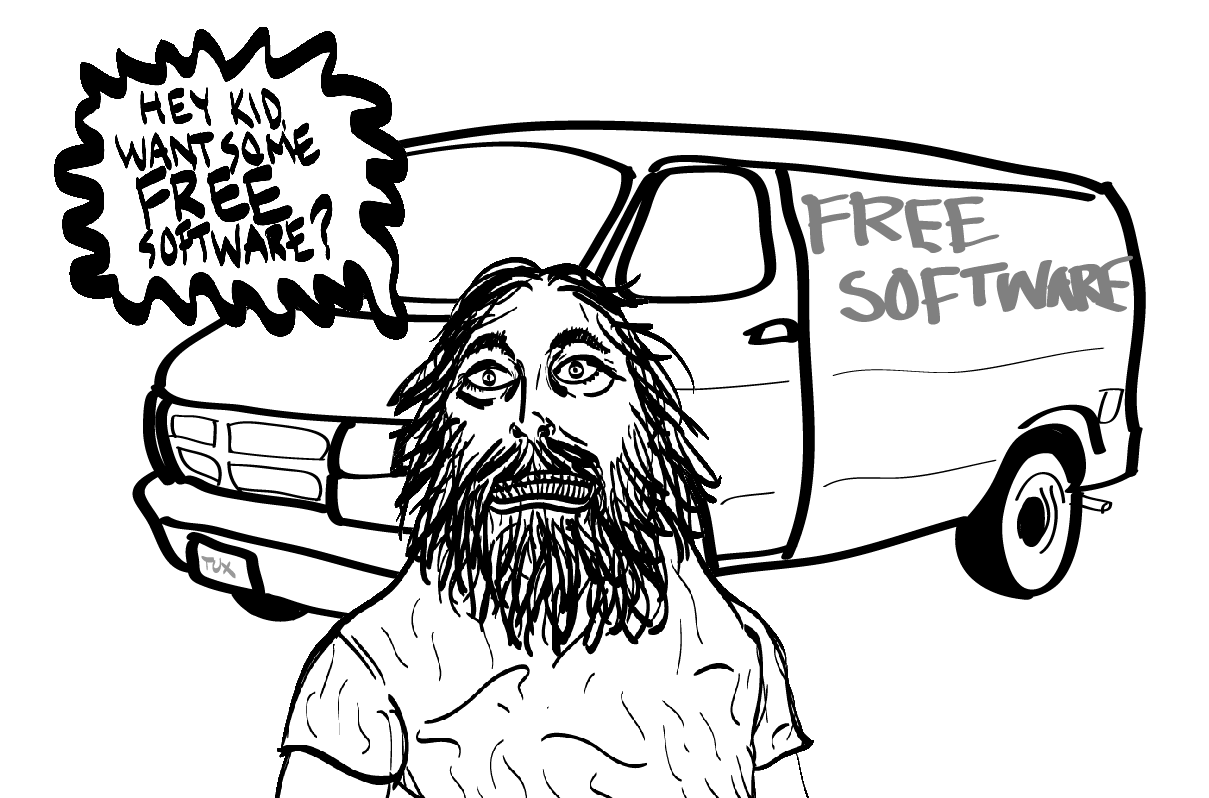
\includegraphics[scale=.35]{./include/gpl.png}
  \caption{The GNU GPL Explained}
  \label{fig:gnu}
\end{figure}
This package is free software licensed under the GNU General Public License, version $\geq$ 2 (see Figure~\ref{fig:gnu}).
If you violate the terms of the GPL then Richard Stallman's beard will sue you in internet court.
